\chapter{Abstração de Imagens} \label{chap:abstracao}

*********

- Falar sobre o filtro gaussiano, image blur;

- Expandir trabalho relacionado;

*********

Neste capítulo é efetuada uma análise das diversas abordagens existentes para a abstração de imagens. Inicialmente, é apresentada uma contextualização da abstração de imagens, no âmbito da estilização artística de imagens, onde são abordadas de forma sumária as diferentes técnicas existentes para o efeito. De seguida, encontram-se descritos alguns dos filtros de abstração de imagens mais comuns. Por último, é ainda apresentado um trabalho relacionado com esta dissertação na área de abstração de imagens.

\section{Estilização Artística de Imagens}
Os conteúdos foto-realistas, possuem muitas vezes mais informação do que a necessária para uma comunicação visual eficaz. A área da Estilização Artística de Imagens (\textit{Image Based Artistic Rendering}), onde se insere a abstração de imagens,  tem como objetivo fazer a transformação de imagens e vídeos foto-realistas 2D em novas formas de representação visual simplificada. A estilização de imagens e vídeos permite, para além da simplificação do conteúdo visual, a sua estruturação de forma a dar ênfase e enfoque a determinadas características das imagens. Desta forma, é possível guiar a perceção obtida dos conteúdos visuais conforme o objetivo da mensagem a comunicar. Por outro lado, estas técnicas permitem criar novas formas de representação gráfica de informação, dotando assim os artistas de novas ferramentas de comunicação e criação de conteúdos visuais.

Atualmente a área da estilização artística de imagens diversificou-se numa atividade multidisciplinar que engloba áreas como a visão por computador, interação humano computador, computação gráfica e a modelação percetual \textit{(perceptual modeling)}. Os sistemas de estilização evoluíram também desde sistemas semi-automáticos de processamento de imagem no início dos anos 90, até sistemas totalmente automáticos de renderização. Adicionalmente o recurso a técnicas de visão por computador e o uso de filtros de abstração de imagens, permitiram melhorias notáveis ao nível da manipulação de grandes quantidades de informação, assim como da informação visual produzida. Uma evolução desta técnicas até atualidade pode ser vista na imagem \ref{fig:arEvolution}.

\begin{figure}[ht]
  \begin{center}
    \leavevmode
    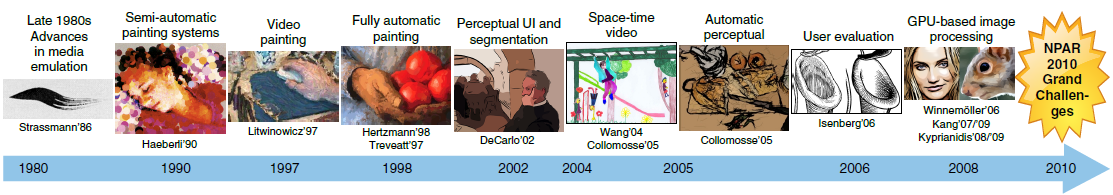
\includegraphics[width=1\textwidth]{arEvolution}
    \caption{Cronologia do desenvolvimento da área da IB-AR \cite{Kyprianidis2012}.}
    \label{fig:arEvolution}
  \end{center}
\end{figure}

De acordo com o estudo do estado da arte da área de estilização artística de imagens e vídeos, realizado por Kyprianidis \textit{et al.} em 2012 \cite{Kyprianidis2012}, as técnicas de estilização existentes podem ser divididas nas seguintes quatro categorias:
\begin{itemize}
\item \textit{Stoke Based Rendering}, as quais criam iterativamente camadas virtuais de traços imitando um pincel, cujas cores, orientação e escala são derivadas de processos automáticos ou semi-automáticos de processamento de imagem; 
\item \textit{Region Based Techniques}, que usam a segmentação da imagem em diversas regiões para a sua posterior estilização;
\item Renderização Baseada em Exemplo, que tentam imitar estilos artísticos específicos através de heurísticas apreendidas para a renderização automática de novas imagens nesses mesmos estilos;
\item Filtros de Abstração de Imagens, os quais usam técnicas de processamento de imagem para, através de operações de filtragem locais, efetuarem a renderização artística e a abstração do conteúdo visual.
\end{itemize}

Apesar de os filtros de abstração de imagens possuírem uma menor diversidade numa perspetiva artística de renderização, a utilização de uma abordagem local por parte destes filtros torna-os vantajosos, quando comparada com as restantes técnicas de renderização artística de imagens. Esta abordagem permite uma fácil adaptação dos processos de abstração de imagens a tecnologias de processamento paralelo, presentes nos CPUs modernos, assim como uma implementação direta do processo de abstração de alguns dos filtros pelos próprios GPUs. Nesse sentido, e devido ao grande número de imagens utilizadas no processo de reconhecimento facial automático a utilização de filtros de abstração de imagens torna-se mais vantajosa no âmbito desta dissertação.

\section{Filtros de Abstração de Imagens}
Os filtros de abstração de imagens permitem simplificar o conteúdo visual, destacando apenas a informação essencial contida nas imagens. Existem vários tipos de filtros de abstração, de seguida encontram-se descritas cinco categorias de filtros de abstração de imagem tipicamente utilizados.
\begin{figure}
        \centering
        \begin{subfigure}[b]{0.3\textwidth}
                \centering
                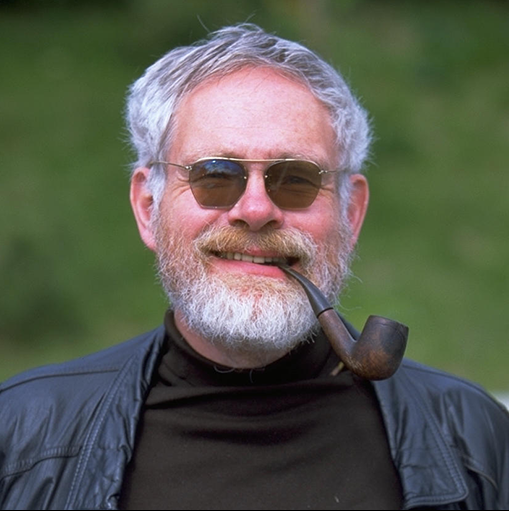
\includegraphics[width=\textwidth]{1-original}
                \caption{Imagem Original}
                \label{fig:original}
        \end{subfigure}%
        ~ %add desired spacing between images, e. g. ~, \quad, \qquad etc.
          %(or a blank line to force the subfigure onto a new line)
        \begin{subfigure}[b]{0.3\textwidth}
                \centering
                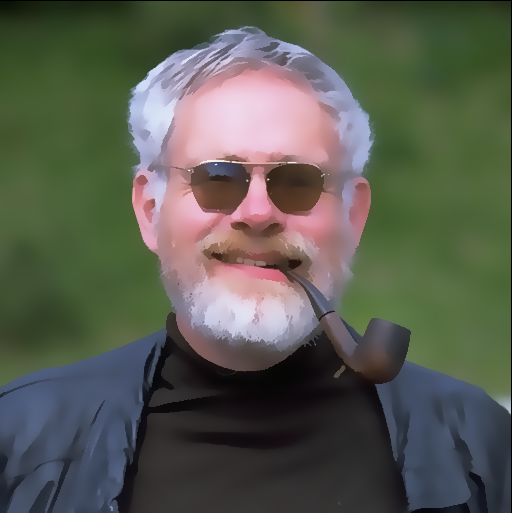
\includegraphics[width=\textwidth]{2-bilateral}
                \caption{Filtro Bilateral}
                \label{fig:bilateral}
        \end{subfigure}
        ~ %add desired spacing between images, e. g. ~, \quad, \qquad etc.
          %(or a blank line to force the subfigure onto a new line)
        \begin{subfigure}[b]{0.3\textwidth}
                \centering
                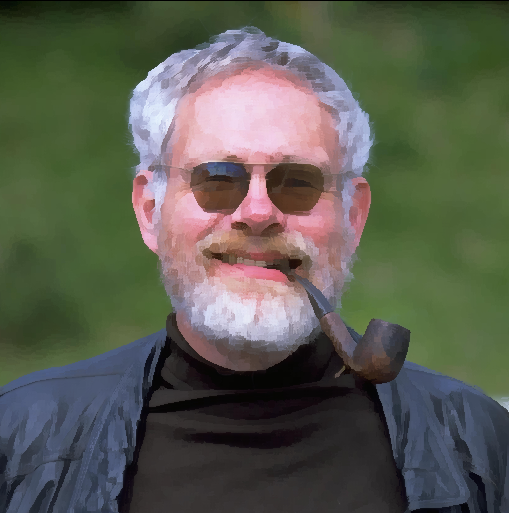
\includegraphics[width=\textwidth]{3-kuwahara}
                \caption{Kuwahara}
                \label{fig:kuwahara}
        \end{subfigure}
        \begin{subfigure}[b]{0.3\textwidth}
                \centering
                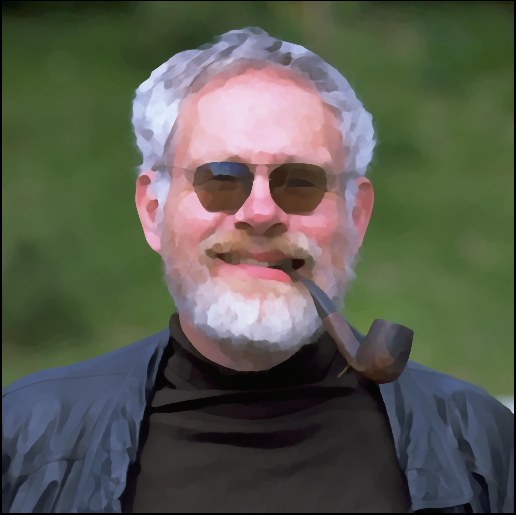
\includegraphics[width=\textwidth]{4-paparietal}
                \caption{Papari \textit{et al.}}
                \label{fig:papari}
        \end{subfigure}
        \begin{subfigure}[b]{0.3\textwidth}
                \centering
                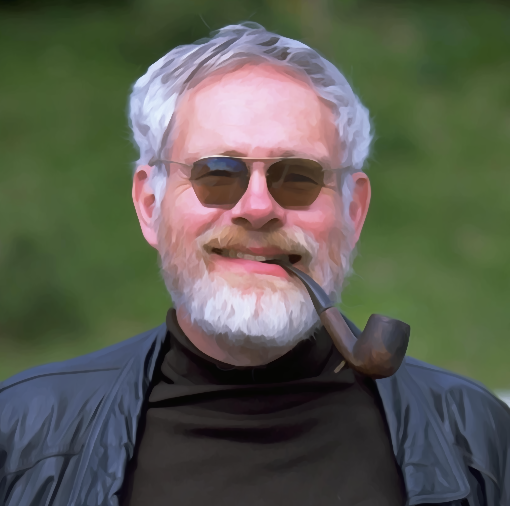
\includegraphics[width=\textwidth]{2-anisotropic}
                \caption{Kuwahara Anisotrópico}
                \label{fig:anisotropic}
        \end{subfigure}
        \caption{Diferentes filtros de abstração aplicados sobre a mesma imagem \cite{Kyprianidis2009}.}\label{fig:filtrosabtracao}
\end{figure}

\subsection{Filtro Bilateral} \label{subsec:bilateral}
Uma abordagem baseada num filtro bilateral foi proposta em primeira mão por Tomasi e Manduchi em 1998 \cite{Tomasi1998} e encontra-se representada na imagem \ref{fig:bilateral}. Já em 2006, Winnemöller propôs uma melhoria dos resultados obtidos através da associação de um filtro de diferença de gaussianas na aplicação do filtro bilateral \cite{Winnemoller2006}. Trabalhos posteriores com vista a melhorar, os contornos produzidos pelas imagens abstraídas foram também realizados com sucesso através da introdução de um filtro de diferença de gaussianas baseado baseado em fluxo \cite{Kang2009}.

O filtro bilateral caracteriza-se por suavizar as zonas com menor contraste da imagem enquanto preserva os limites de maior contraste. No entanto, os efeitos deste filtro são poucos visíveis quando toda a imagem possui um elevado contraste. Por outro lado, em imagens pouco contrastadas a informação visual removida é por vezes demasiada, causando um efeito de imagem desfocada na imagem abstraída.

\subsection{Kuwahara} \label{subsec:kuwahara}
O filtro Kuwahara(fig. \ref{fig:kuwahara}) e as suas variantes, representam uma classe de filtros onde se tem verificado uma pesquisa ativa ao longo das últimas décadas \cite{Kyprianidis2009}.

A ideia geral do filtro do tipo Kuwahara consiste em efetuar um achatamento da imagem, através da divisão da área a filtrar em quatro sub-regiões retangulares de menor dimensão e a posterior substituição da informação contida numa dessas regiões pela média da sub-região com menor variância. Desta forma, é removido o detalhe em zonas com elevado contraste mas são preservadas as limites das formas presentes na imagem. No entanto, na presença de ruído este filtro revela-se instável, criando artefactos na imagem. Para além disso, esta abordagem revela-se também agressiva na presença de anisotropia \footnote{Anisotropia - qualidade de certos materiais cujas propriedades são diferentes consoante as direções.}, ou seja quando a informação direcional presente na imagem é forte (por exemplo: pelo, cabelos), não preservando essa informação na imagem abstraída.

Existem várias variantes ao filtro Kuwahara, sendo que a grande diferença entre a maior parte das variantes consiste na forma como são definidas as sub-regiões a filtrar. Papari \textit{et al.} \cite{Papari2007}, apresentaram, com bons resultados, uma variante deste filtro em que a divisão das sub-regiões é efetuada em regiões circulares, que por sua vez se encontram divididas em oito regiões de igual tamanho. Apesar das melhorias registadas na abordagem de Papari \textit{et al.}, visíveis na figura \ref{fig:papari}, esta abordagem continua a não preservar a informação direcional contida nas imagens resultando assim no aparecimento de alguns artefactos, ainda que mais pequenos e com maior definição do que na solução proposta pelo o filtro original.

Para ultrapassar as limitações do filtro Kuwahara original na presença de anisotropia, foi proposta por Kyprianidis \textit{et al.} \cite{Kyprianidis2009}, uma nova abordagem com o nome filtro Kuwahara Anisotrópico (\ref{fig:anisotropic}). Nesta solução, é feita uma adaptação da forma, orientação e escala do método de seleção das sub-regiões à estrutura local da imagem, resultando numa forma que varia entre um círculo e um elipse alongada conforme a própria estrutura local da imagem. Assim, para além de preservada, a informação direcional é ainda enfatizada, resultando em imagens tipo pintura, com limites bem definidos e sem grandes artefactos visíveis.

\subsection{\textit{Diffusion Shock Filter}}
\begin{figure}
        \centering
        \begin{subfigure}[b]{0.3\textwidth}
                \centering
                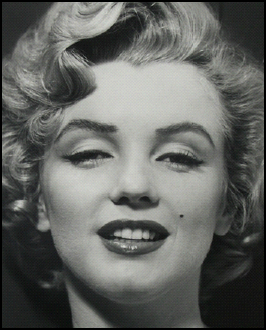
\includegraphics[width=\textwidth]{monroe_original}
                \caption{Imagem Original}
                \label{fig:monroe_original}
        \end{subfigure}%
        ~ %add desired spacing between images, e. g. ~, \quad, \qquad etc.
          %(or a blank line to force the subfigure onto a new line)
        \begin{subfigure}[b]{0.3\textwidth}
                \centering
                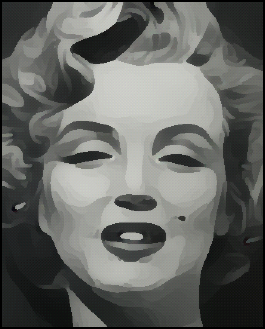
\includegraphics[width=\textwidth]{monroe_abstraida}
                \caption{Resultado Abstração}
                \label{fig:monroe_abstraida}
        \end{subfigure}
        \caption{\textit{Diffusion Shock Filter} \cite{Kang2008}.}\label{fig:diffusion_shock_filter}
\end{figure}
Kang e Lee \cite{Kang2008}, foram os primeiros a utilizar \textit{shock filtering} para a abstraçao de imagens através do uso de \textit{Mean Curvature Flow (MCF)}, resultando em imagens onde para além de suavizadas as variações irrelevantes das cores, são simplificados os limites das formas presentes nas mesmas, como é possível visualizar na figura \ref{fig:diffusion_shock_filter}. O resultando da aplicação de \textit{shock filtered MFC}, é, no entanto, tipicamente é muito agressivo, resultando em imagens desfocadas, onde apenas é parcialmente preservada a  informação direcional contida na imagem. Esta técnica revela-se também, pouco indicada para a abstração de vídeo, uma vez que é pouco sensível a pequenas alterações nas imagens.

\subsection{Filtros Morfológicos}
Os filtros desta categoria, utilizam os princípios da morfologia matemática para reduzir o detalhe existente nas zonas coloridas, criando um efeito de uniformização da cor. A morfologia matemática foi introduzida originalmente por Matheron and Serra em 1982 \cite{serra1982image}, e consiste numa teoria para a análise e processamento de estruturas geométricas. De uma forma geral maioria das operações morfológicas são baseadas em simples operações de expansão e encolhimento e são designadas dilatação e erosão.

Existe uma grande variedade de abordagens e filtros baseados nos princípios da morfologia matemática, existindo consequentemente uma grande variedade ao nível dos resultados obtidos, conforme o filtro morfológico aplicado.

\subsection{Técnicas \textit{Gradient Domain}}
O gradiente de uma imagem representa de forma direcional as mudanças de intensidade de uma imagem independente das suas cores originais, permitindo assim uma maior flexibilidade na manipulação das imagens. As técnicas baseadas no uso de gradientes, consistem na construção de um campo de gradiente que representa a imagem, o qual é posteriormente utilizado na reconstrução da imagem filtrada.

A grande desvantagem das técnicas baseadas no uso de gradientes é que os resultados obtidos em zonas com contraste são por vezes problemáticos e requerem correção. Para além disso, a computação deste tipo de filtragem é computacionalmente pesada e por isso não aplicável para situações de utilização em tempo real.

\section{Trabalho Relacionado}
Os filtros de abstração são normalmente utilizados por artistas para comunicar a mensagem visual mais eficazmente.  No âmbito desta dissertação pretendemos analisar o impacto destes filtros não ao nível da comunicação visual efetuada, mas ao nível do impacto que estes podem causar no processo de reconhecimento facial. Esta investigação é motivada por resultados anteriores obtidos com o uso dos mesmos filtros na ilustração automática de texto.

A ilustração de texto é uma tarefa enquadrada na área da recuperação de informação multimédia e que consiste na pesquisa de imagens adequadas para a ilustração de fragmentos de texto, tais como notícias ou livros. Coelho e Ribeiro  \cite{Coelho:2012:IAC:2260641.2260676}, propõem o uso da abstração de imagens para a ilustração automática de texto, através de um sistema de recuperação de informação, o qual dada uma entrada textual inicial, seleciona automaticamente uma pequena lista de imagens relacionadas a partir da análise coleção de imagens previamente processada.

O sistema desenvolvido utiliza a abstração de imagens para melhorar a informação capturada pelos descritores de informação visual utilizados e consequentemente melhorar os resultados obtidos a partir da análise baseada em conteúdos efetuada à coleção de dados.

Os resultados obtidos demonstraram que o uso de abstração tem a potencialidade de melhorar a informação recuperada, assim como reduzir as necessidades de processamento e armazenamento da coleção de dados utilizada.